%!TEX program = xelatex
\documentclass[8pt, landscape, a4paper]{extarticle}

% --- 核心宏包 ---
\usepackage[UTF8, fontset=fandol]{ctex}
\usepackage[margin=0.8cm, top=1cm, bottom=1.3cm]{geometry}
\usepackage{multicol}
\usepackage{xcolor}
\usepackage{tcolorbox}
\usepackage{enumitem}
\usepackage{amsmath}
\usepackage{amssymb}
\usepackage{fontspec}
\usepackage{tikz}
\usetikzlibrary{arrows.meta, shapes}

% --- 去掉页码 ---
\pagestyle{empty}

% --- 颜色定义 (Dark Green 主题) ---
\definecolor{headerblue}{RGB}{20, 90, 50}      % Dark Green
\definecolor{navcolor}{RGB}{211, 84, 0}        % 导航橙
\definecolor{intuitioncolor}{RGB}{41, 128, 185}% 直觉蓝
\definecolor{accentcolor}{RGB}{192, 57, 43}    % 强调红
\definecolor{section2}{RGB}{142, 68, 173}      % 紫色
\definecolor{dividergray}{RGB}{220, 220, 220}

% --- 全局设置 ---
\setlength{\parindent}{0pt}
\setlength{\columnsep}{0.4cm} 
\linespread{1.1} 

% --- 列表样式 ---
\setlist[itemize]{leftmargin=1.2em, nosep, itemsep=2pt, topsep=2pt, label=$\textcolor{headerblue}{\vcenter{\hbox{\tiny$\bullet$}}}$ }
\setlist[description]{leftmargin=0.2em, style=sameline, nosep, itemsep=2pt, font=\bfseries}

% --- Box 样式 ---
\newtcolorbox{mybox}[2][]{%
  colback=white,
  colframe=#2,
  coltitle=white,
  boxrule=1pt,             
  arc=2mm,                 
  left=4pt, right=4pt, top=3pt, bottom=3pt, 
  toptitle=3pt, bottomtitle=3pt, 
  fonttitle=\bfseries\sffamily\large,
  title={#1},
  after skip=5pt          
}

% --- 自定义命令 ---
\newcommand{\subt}[1]{{\vspace{2pt}\textbf{\large \textcolor{black}{#1}}}}

\newcommand{\boxdesc}[1]{%
    \textit{\small \textcolor{gray}{#1}}%
    \par\vspace{2pt}%
    {\color{dividergray}\hrule height 0.5pt}%
    \vspace{2pt}%
}

\newcommand{\sepline}{%
    \par \vspace{3pt}%
    {\color{dividergray}\hrule height 0.5pt}%
    \par \vspace{3pt}%
}

% 公式间距
\setlength{\abovedisplayskip}{3pt}
\setlength{\belowdisplayskip}{3pt}

\begin{document}

% --- 页眉 ---
\begin{center}
    {\Huge \textbf{\sffamily \textcolor{headerblue}{辛几何 Symplectic Geometry Cheat Sheet}}} \\
    \vspace{0.2cm}
    {\large \texttt{The Geometry of Phase Space: Mechanics and Area Preservation}}
\end{center}

% --- 开始四栏布局 ---
\begin{multicols*}{4}

% === 第一栏 ===

\begin{mybox}[️ 场景导航 (Use Cases)]{navcolor}
    \boxdesc{遇到什么问题 $\to$ 用什么工具}
    \begin{itemize}[itemsep=2pt]
        \item \textbf{经典力学} $\to$ 哈密顿方程 / 相空间
        \item \textbf{数值积分 (保能量)} $\to$ 辛积分器 (Symplectic Integrator)
        \item \textbf{量子化} $\to$ 几何量子化 / 形变量子化
        \item \textbf{光学} $\to$ 费马原理 / 辛矩阵
        \item \textbf{镜像对称} $\to$ 凯勒流形 (Kähler)
        \item \textbf{控制理论} $\to$ 庞特里亚金极值原理
    \end{itemize}
\end{mybox}

\begin{mybox}[1. 辛向量空间 (Linear)]{headerblue}
    \boxdesc{反对称的内积}
    
    \subt{辛形式 $\omega$}
    向量空间 $V$ 上的双线性形式,满足:
    \begin{itemize}
        \item \textbf{反对称}: $\omega(u, v) = -\omega(v, u)$。
        \item \textbf{非退化}: $\forall u \neq 0, \exists v, \omega(u, v) \neq 0$。
    \end{itemize}
    \textit{推论: $V$ 的维数必须是偶数 $2n$。}
    \sepline
    
    \subt{标准型}
    存在基底 $\{q_i, p_i\}$ 使得:
    $$ \omega = \sum_{i=1}^n dp_i \wedge dq_i $$
    \textit{物理意义: $q$ 是位置,$p$ 是动量。$\omega$ 测量“有向面积”。}
\end{mybox}

\begin{mybox}[2. 辛流形 (Manifold)]{headerblue}
    \boxdesc{弯曲的相空间}
    
    \subt{定义 $(M, \omega)$}
    $M$ 是偶数维流形,$\omega$ 是闭的非退化 2-形式。
    $$ d\omega = 0 $$
    \sepline
    
    \subt{达布定理 (Darboux)}
    辛流形在\textbf{局部}都和标准辛空间 $(\mathbb{R}^{2n}, \sum dp_i \wedge dq_i)$ 同构。
    \textit{对比: 黎曼流形局部有曲率,辛流形局部都是平的。辛几何是全局几何。}
    \sepline
    
    \subt{余切丛 (Cotangent Bundle)}
    $M = T^*Q$ 具有典范辛形式 $\omega = d\theta$ (刘维尔形式)。
\end{mybox}

\columnbreak

% === 第二栏 ===

\begin{mybox}[3. 哈密顿力学 (Hamiltonian)]{headerblue}
    \boxdesc{物理的几何化}
    
    \subt{哈密顿向量场 $X_H$}
    给定能量函数 (哈密顿量) $H: M \to \mathbb{R}$,定义 $X_H$:
    $$ \iota_{X_H} \omega = dH $$
    即 $\omega(X_H, \cdot) = dH(\cdot)$。
    \sepline
    
    \subt{运动方程}
    $$ \dot{q} = \frac{\partial H}{\partial p}, \quad \dot{p} = - \frac{\partial H}{\partial q} $$
    这正是 $X_H$ 的积分曲线。
    \sepline
    
    \subt{刘维尔定理 (Liouville)}
    哈密顿流保持辛形式 $\omega$ 不变 (也保持体积形式 $\omega^n$ 不变)。
    \textit{物理意义: 相空间体积守恒 (信息不灭)。}
    \sepline
    
    \subt{诺特定理 (Noether)}
    若 $H$ 在辛变换 $\phi_t$ 下不变,则生成元 $f$ 是守恒量。
    $$ \{f, H\} = 0 \implies f \text{ 是运动常数} $$
\end{mybox}

\begin{mybox}[4. 泊松括号 (Poisson Bracket)]{headerblue}
    \boxdesc{代数结构}
    
    \subt{定义}
    $$ \{f, g\} = \omega(X_f, X_g) $$
    在标准坐标下:
    $$ \{f, g\} = \sum (\frac{\partial f}{\partial q_i}\frac{\partial g}{\partial p_i} - \frac{\partial f}{\partial p_i}\frac{\partial g}{\partial q_i}) $$
    \sepline
    
    \subt{演化方程}
    $$ \frac{df}{dt} = \{f, H\} $$
    \textit{量子力学对应: $\frac{d\hat{A}}{dt} = \frac{1}{i\hbar} [\hat{A}, \hat{H}]$。}
    \sepline
    
    \subt{雅可比恒等式 (Jacobi)}
    $$ \{f, \{g, h\}\} + \{g, \{h, f\}\} + \{h, \{f, g\}\} = 0 $$
    \textit{这使得光滑函数空间构成无穷维李代数。}
\end{mybox}

\columnbreak

% === 第三栏 ===

\begin{mybox}[5. 辛积分器 (Symplectic Integrator)]{headerblue}
    \boxdesc{数值计算的魔法}
    
    \subt{为什么不用 RK4?}
    普通积分器 (如 Runge-Kutta) 不保持辛结构,长期积分会导致能量漂移 (系统发散或耗散)。
    \sepline
    
    \subt{Verlet / Leapfrog 算法}
    $$ p_{n+1/2} = p_n - \frac{\Delta t}{2} \nabla V(q_n) $$
    $$ q_{n+1} = q_n + \Delta t M^{-1} p_{n+1/2} $$
    $$ p_{n+1} = p_{n+1/2} - \frac{\Delta t}{2} \nabla V(q_{n+1}) $$
    \textit{特性: 显式、时间可逆、长期保持能量稳定。}
    \sepline
    
    \subt{影子哈密顿量 (Shadow Hamiltonian)}
    辛算法精确求解的是一个被扰动的哈密顿量 $\tilde{H} = H + O(\Delta t^k)$。
\end{mybox}

\begin{mybox}[6. 拉格朗日流形 (Lagrangian)]{headerblue}
    \boxdesc{半维子流形}
    
    \subt{定义 $L \subset M$}
    $L$ 的维数是 $M$ 的一半 ($n$),且 $\omega|_L = 0$。
    \textit{例子: 构型空间 (只包含 $q$ 的空间) 是相空间的一个拉格朗日子流形。}
    \sepline
    
    \subt{应用}
    WKB 近似、焦散线 (Caustics)、几何光学。
    \sepline
    
    \subt{生成函数 (Generating Function)}
    辛变换可以通过生成函数 $S(q, P)$ 隐式定义。
    $$ p = \frac{\partial S}{\partial q}, \quad Q = \frac{\partial S}{\partial P} $$
\end{mybox}

\begin{mybox}[7. Python / SciPy 实战]{headerblue}
    \boxdesc{代码工具箱}
    \begin{itemize}
        \item \textbf{Hamiltonian Monte Carlo (HMC)}:
        利用哈密顿动力学在概率分布上高效采样 (PyMC3 / Stan)。
        \item \textbf{Rebound}: 天体物理辛积分库。
    \end{itemize}
\end{mybox}

\columnbreak

% === 第四栏 ===

\begin{mybox}[8. 高阶前沿 (Advanced)]{headerblue}
    \boxdesc{深水区}
    
    \subt{格罗莫夫非挤压定理 (Non-squeezing)}
    辛骆驼定理:你不能把一个大球通过保辛变换塞进一个细管子里,除非管子够粗。
    \sepline
    
    \subt{Floer 同调}
    无穷维莫尔斯理论。用于证明阿诺德猜想 (哈密顿系统不动点个数)。
    \sepline
    
    \subt{接触几何 (Contact Geometry)}
    奇数维的辛几何对应物。
    \sepline
    
    \subt{深谷范畴 (Fukaya Category)}
    对象是拉格朗日子流形,态射是拉格朗日交。
\end{mybox}

\vspace*{\fill}

\begin{mybox}[ 核心直觉 (Intuition)]{intuitioncolor}
    \boxdesc{“面积是有方向的。”}
    
    % TikZ 矢量图: 相空间流 (面积守恒)
    \begin{center}
    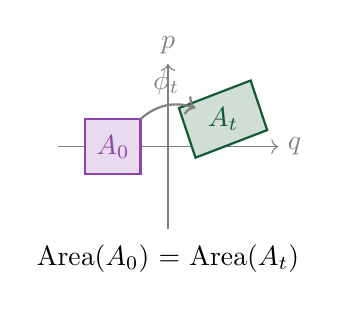
\begin{tikzpicture}[scale=0.7]
        % 坐标轴
        \draw[->, gray] (-2,0) -- (2,0) node[right] {$q$};
        \draw[->, gray] (0,-1.5) -- (0,1.5) node[above] {$p$};
        
        % 初始区域 A
        \draw[thick, section2, fill=section2!20] (-1.5, -0.5) rectangle (-0.5, 0.5);
        \node[section2] at (-1, 0) {$A_0$};
        
        % 演化后的区域 A_t
        \draw[thick, headerblue, fill=headerblue!20] (0.5, -0.2) -- (1.8, 0.3) -- (1.5, 1.2) -- (0.2, 0.7) -- cycle;
        \node[headerblue] at (1, 0.5) {$A_t$};
        
        % 箭头
        \draw[->, thick, gray, bend left] (-0.5, 0.5) to node[midway, above] {$\phi_t$} (0.5, 0.7);
        
        % 注解
        \node[below] at (0, -1.6) {Area($A_0$) = Area($A_t$)};
    \end{tikzpicture}
    \end{center}

    \hspace{1em}辛几何是\textbf{相空间}的几何学。它描述了守恒系统如何随时间演化。
    \vspace{4pt}
    
    \subt{三大核心视角}
    \begin{itemize}[itemsep=4pt]
        \item \textbf{反对称性}: 
        黎曼几何基于对称的度量 $g_{ij}$ (长度),辛几何基于反对称的形式 $\omega_{ij}$ (面积)。
        
        \item \textbf{守恒律}: 
        辛变换不仅保持体积 (Liouville),还保持每个 2D 投影面的有向面积。这比单纯的体积守恒要强得多。
        
        \item \textbf{刚性 (Rigidity)}: 
        辛流形像是一种“不可压缩的流体”,但比流体更硬。有些形状变换在拓扑上允许,在体积上允许,但在辛几何中被禁止 (辛骆驼)。
    \end{itemize}
    
    \vspace{6pt}
    \centering\textit{\footnotesize 动量与位置共舞,面积永恒不变。}
\end{mybox}

\end{multicols*}

\end{document}
